\documentclass[a4paper]{article}
\usepackage{natbib,alifeconf}

\usepackage{subfig}
\usepackage{xcolor}
\usepackage{fancybox}
%Fancy List
\definecolor{solarized@base03}{HTML}{002B36}
\definecolor{solarized@base02}{HTML}{073642}
\definecolor{solarized@base01}{HTML}{586e75}
\definecolor{solarized@base00}{HTML}{657b83}
\definecolor{solarized@base0}{HTML}{839496}
\definecolor{solarized@base1}{HTML}{93a1a1}
\definecolor{solarized@base2}{HTML}{EEE8D5}
\definecolor{solarized@base3}{HTML}{FDF6E3}
\definecolor{solarized@yellow}{HTML}{B58900}
\definecolor{solarized@orange}{HTML}{CB4B16}
\definecolor{solarized@red}{HTML}{DC322F}
\definecolor{solarized@magenta}{HTML}{D33682}
\definecolor{solarized@violet}{HTML}{6C71C4}
\definecolor{solarized@blue}{HTML}{268BD2}
\definecolor{solarized@cyan}{HTML}{2AA198}
\definecolor{solarized@green}{HTML}{859900}
\definecolor{solarized@darkgreen}{HTML}{006400}

\usepackage{listings}

\lstset{
    language=python,
    columns=fixed,
    tabsize=2,
    extendedchars=true,
    breaklines=true,
    frame=single,
    numbers=left,
	numberstyle=\tiny,
    numbersep=5pt,
    rulesepcolor=\color{solarized@base03},
    numberstyle=\tiny\color{solarized@base1},
    basicstyle=\footnotesize\ttfamily,
    keywordstyle=\color{magenta},
    stringstyle=\color{solarized@base00}\ttfamily,
    identifierstyle=\color{solarized@blue},
    commentstyle=\color{solarized@base1},
    emphstyle=\color{solarized@red},
    backgroundcolor=\color{solarized@base3},
    literate={ö}{{\"o}}1
    {ä}{{\"a}}1
    {ü}{{\"u}}1
    {Ö}{{\"O}}1
    {Ä}{{\"A}}1
    {Ü}{{\"U}}1
}
\lstset{
 morekeywords={OPTIONS, TITLE, LET, PROC, SURVEYSELECT, NOPRINT, SORT, MEANS, DATA, MEND, MACRO, RUN, SQL, QUIT, UNIVARIATE, SURVEYMEANS, SELECT, INTO, FROM, PUT,BY,SET,VAR,OUTPUT,SAMPRATE,REP,SEED, STRATA,ALLOC,END,IF,THEN,ELSE,MERGE,KEEP,RENAME,DO,HISTOGRAM,OUT,METHOD,STATS,RATE,WEIGHT,STATISTICS,ODS, MEAN,SUM},
 moredelim=[is][\color{solarized@darkgreen}]{|}{|}
 morecomment={total}
}


\pagenumbering{roman}


\title{Bootstrapping the Support Vector Machine}

\author{Thomas Goerttler$^{1,2,3}$, Christian Koopmann$^{1,2,3}$, Patricia Craja$^{1,2,3}$ \\
\mbox{}\\
$^1$Humboldt University of Berlin, Unter den Linden 6, 10099 Berlin \\
$^2$Free University Berlin, Kaiserswerther Str. 16-18, 14195 Berlin \\
$^3$Technical University of Berlin, 10623 Berlin \\
thomas.goerttler@gmail.com\\
c.k.e.koopmann@gmail.com\\
Patricia.craja@gmx.de\\
}


\begin{document}
\maketitle

\begin{abstract}
The goal of this project is to apply the bootstrap method to support vector machines (SVMs) in order to estimate the uncertainty of the prediction rule constructed with training samples. We found a way to calculate the variance of SVMs and therefore use parallelization. Moreover we will show how this uncertainty is correlated with other aspects of the SVM, such as the tuning parameter, the balance of the training data and the number of support vector machines. We analyze this impact for both linear and Gaussian Kernel SVMs.
  
\end{abstract}

\section{Introduction}

	Support Vector Machines are one of the most successful methods of Machine Learning. SVMs have many merits that distinguish them from many other machine learning algorithms, including the nonexistence of local minima, the speed of calculation, and the use of only two tuning parameters. Given a binary training data set, an SVM learning algorithm builds a model that predicts the unknown class for new input data, making it a non-probabilistic binary linear classifier. SVM is based on a minimization problem, which seeks for a hyperplane in the feature space that optimally separates data points of two clusters.  By reducing non-linear complex decisions problems to linear problems through application of the Kernel-Trick, they represent a computationally efficient way to tackle these problems. The dimension of the feature space is controlled by the choice of a specific Kernel function. Common Kernels are the linear Kernel, the Gaussian Kernel (RBF) and the Polynomial Kernel.
    SVMs based on certain Kernels (e.g. Gaussian RBF Kernel) are non parametric methods. Since the distribution of the underlying data is generally unknown so is the finite sample distribution of these methods. 
There has been considerable research on the asymptotic distribution of SVMs, which have been shown to be asymptotically normally distributed under certain conditions. An alternative idea to estimate these distributions is to use Efrons empirical boot- strap. The idea behind this method is to repeatedly draw samples with replacement from the full data according to the empirical distribution function of the data. Through the repeated calculation of the statistic of interest one can get an estimate of its distribution. For the SVM this estimate has been shown to be consistent under relatively mild conditions.
    
 


\section{Problem}
  In contrast to probabilistic classifiers which provide classification with a degree of certainty, SVMs only predict the most likely class that the sample should belong to.  
Since no adequate distribution theory exists, we provide bootstrapping method to the SVM algorithm to calculate the variance of its predictions. Given the variance, we changed different parameters such as
the tuning parameter, the data-distribution and SVM attributes in order to analyze the influence of these parameters on the variance.

Because predictions are only binary variables and therefore might be identical across all bootstrap samples we use minimal distance of prediction point to decision boundary as real valued substitute. 



\begin{figure}[!htb]
\begin{center}
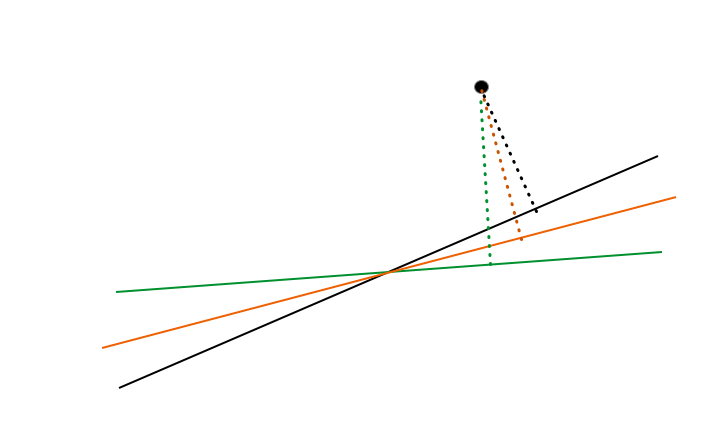
\includegraphics[width=1.5in]{abb/distances.jpg}
\caption{Really awesome trick of distance}
\label{fig1}
\end{center}
\end{figure}

\begin{figure}[!htb]
\begin{center}
\subfloat[]{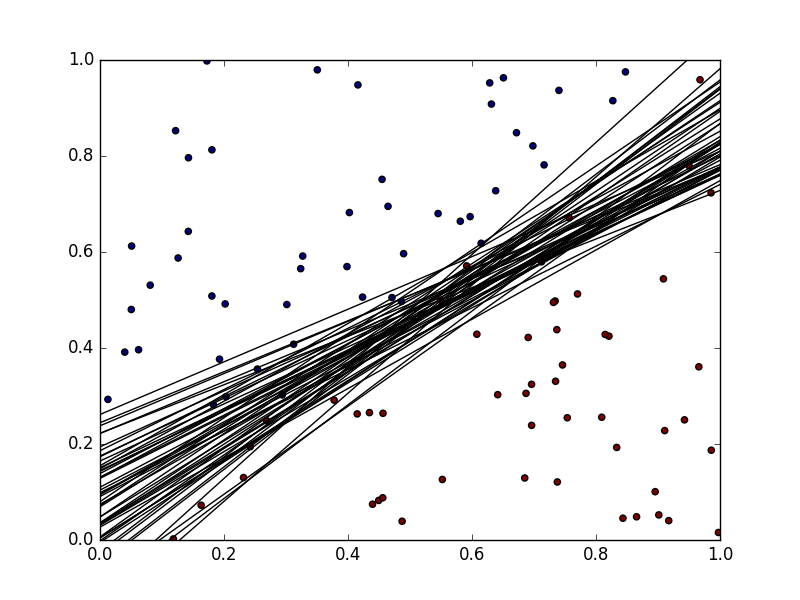
\includegraphics[width=1.5in]{abb/100_n.jpg}}
\subfloat[]{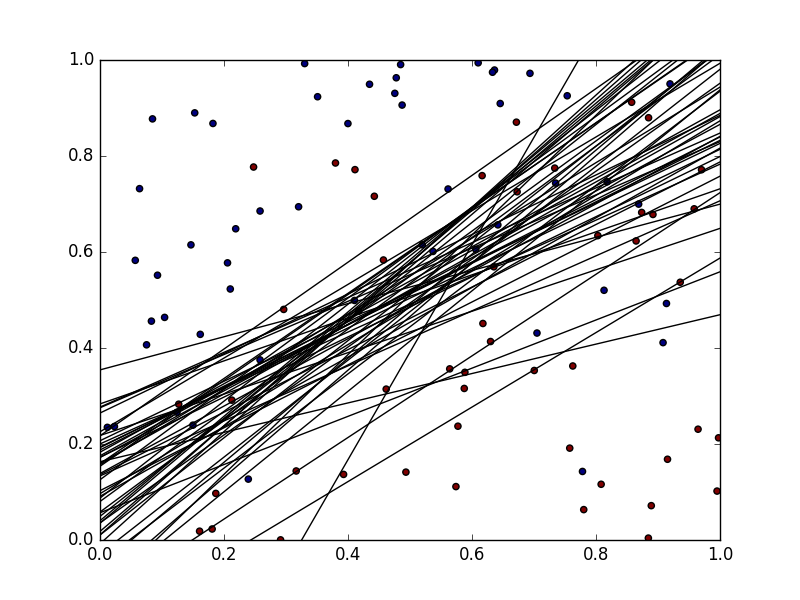
\includegraphics[width=1.5in]{abb/100_y.jpg}}

\subfloat[]{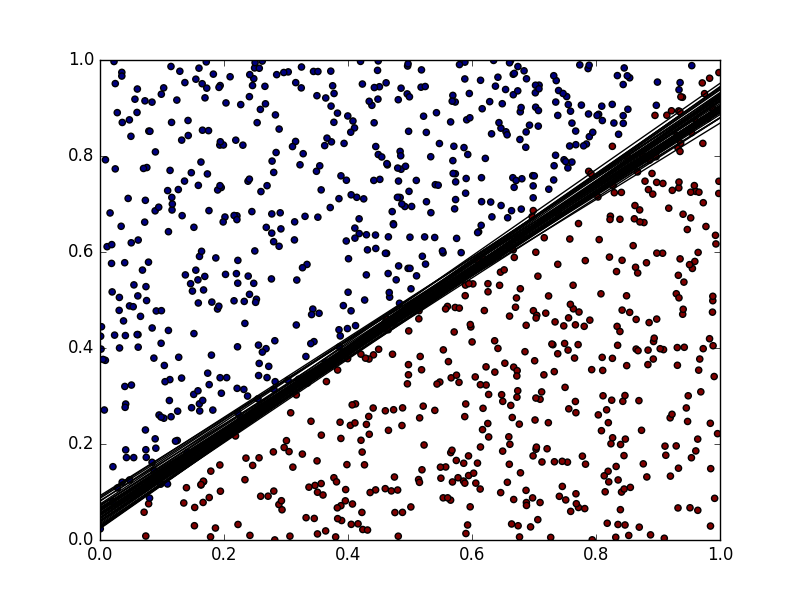
\includegraphics[width=1.5in]{abb/1000_n.jpg}}
\subfloat[]{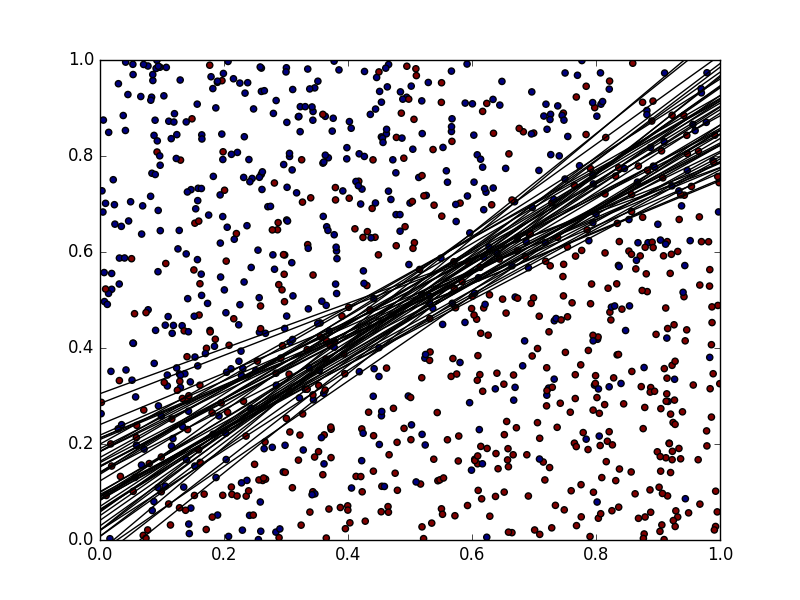
\includegraphics[width=1.5in]{abb/1000_y.jpg}}
\caption{(a) They are 100 perfectly seperated points, (b) They are 100 not perfectly seperated points ...... }
\label{fig1}
\end{center}
\end{figure}


\section{Implementation}



\begin{figure}[!htb]
\begin{center}
\begin{lstlisting}
def bootstrap_the_svm(trainings_data, prediction_data, kernel, C, gamma = "auto", degree = 3, processes = 10, replications = 1000):

    input_parameters = SVM_Input(trainings_data, prediction_data, kernel, C, gamma, degree)
    data = input_parameters
    real_svm = do_svm(data)
    
    ### Do bootstrapping
    PROCESSES = processes
    REPLICATIONS = replications
    pool = Pool(processes = PROCESSES)
    results = pool.map(single_sample_and_svm, [data] * REPLICATIONS)
        
    ### Calculate the Variance of the Support Vector Machine
    
    points_information = Points_Information(results)
    
    variance_of_svm_probabilites = calculate_variance_of_svm(points_information.probabilites)
    variance_of_svm_distance_to_hyperplane = calculate_variance_of_svm(points_information.distances)
    
    result = Bootstrap_Result([real_svm[0], real_svm[1], real_svm[2], variance_of_svm_probabilites, variance_of_svm_distance_to_hyperplane], real_svm[0].n_support_ )
        
    return(result)
\end{lstlisting}
\caption{Implementation of Bootstrapping}
\label{fig1}
\end{center}
\end{figure}
\subsection{Bootstrapping}
In order to calculate the variance of the predictions we use bootstrap samples. We start by training the SVM on the full training data. Then we draw N random bootstrap samples with replacement from the full training data and train the SVM N times on each bootstrap sample in a parallelized manner. That way we get N different SVMs, on which we can apply the test data set. For each SVM, we return the distance of each point in the test data set from the decision boundary.  Finally we can calculate the variance of distances for each point in the test data set. We take the average of these N Variances as an indicator for the variance of the prediction rule. Therefore our Bootstrap Method uses as Input the training data set, the test data set, SVM-Parameters, and the amount N of bootstrap replications and it returns the Full SVM as well as the variance of test data distances.

\begin{figure}[!htb]
\begin{center}
\begin{lstlisting}
def get_data_normaly_distributed(coefs, errorCoef, intercept, size):
	inputs = []
	error = errorCoef*rd.standard_normal(size)
	y = error + intercept
	for i in range(len(coefs)):
		 inputs = inputs + [rd.standard_normal(size)]		 
		 y = y+coefs[i]*inputs[i]
	y = sign(y)
	inputs = list(zip(*inputs))
	return([y,inputs])
\end{lstlisting}
\caption{Implementation of Datasimulation normally distributetd}
\label{fig1}
\end{center}
\end{figure}
\subsection{Data Simulation}
For the Data Simulation we use two different approaches, the Hyperplane- and the Centroid- Approach. For both we assume to randomly draw $n$ observations for the input variables $x$ from a normal distribution. The Hyperplane-Approach calculates the labels using the formula $y= sign(c+ w^T x + error)$, given the Hyperplane parameter $w$, a constant $c$ as well as the error distribution, whereas the Centroid-Approach calculates the labels using the formula $y= sign(c + a_1*(d(x,z_1)^{-1}... + error)$ given the Centroid- Locations $z_i$, the Centroid- Parameters  $a_i$, a constant $c$ and a distance function $d(a,b)$.


\begin{figure}[!htb]
\begin{center}
\begin{lstlisting}
def get_data_centroid_distributed(coefs, locations, errorCoef, size, intercept, distance, xdistribution = "normal", par1 = 0, par2 = 1):
	X = []
	dimension = len(list(zip(*locations)))
	for i in range(dimension):
		if(xdistribution == "normal"):		
			X = X + [rd.normal(par1, par2, size)]
		elif(xdistribution == "uniform"):
			X = X + [rd.uniform(par1, par2, size)]
		else:
			print("Please choose supported Distribution")
			return None	
	X = list(zip(*X))
	distances = []
	error = errorCoef*rd.standard_normal(size)
	y = error + intercept
	for i in range(size):	
		newDistance = pdist([X[i]]+locations, distance)
		newDistance = newDistance[:len(locations)]
		inverseDistance = power(newDistance, -1)
		y[i] = y[i] + dot(coefs, inverseDistance)
		distances = distances + [newDistance]
	y = sign(y)
	#distances = list(zip(*distances))
	return([y,X])	
	
\end{lstlisting}
\caption{Implementation of Datasimulation normally distributetd}
\label{fig1}
\end{center}
\end{figure}




\section{Results}

In this section we will show how the prediction variance is correlated with other aspects of the SVM, such as the tuning parameter $C$, the balance of the training data and the number of support vectors of the original Full-SVM. Analyzing this impact for both linear and Gaussian Kernel SVMs we found following interesting results:


\subsection{Influence of the tuning parameter C}
Kernels are powerful! Kernels are powerful! Kernels are powerful! Kernels are powerful! Kernels are powerful! Kernels are powerful! Kernels are powerful! Kernels are powerful! Kernels are powerful! Kernels are powerful! Kernels are powerful! Kernels are powerful! Kernels are powerful! Kernels are powerful! Kernels are powerful! Kernels are powerful! Kernels are powerful! Kernels are powerful! Kernels are powerful! Kernel
 

\begin{figure}[!htb]
\begin{center}
\subfloat[]{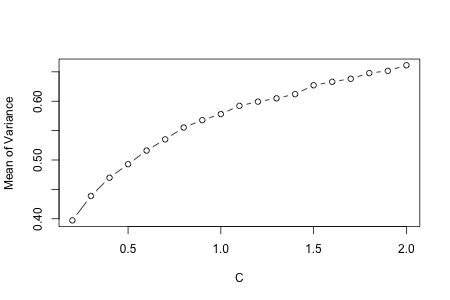
\includegraphics[width=3in]{abb/c_lin.jpg}}

\subfloat[]{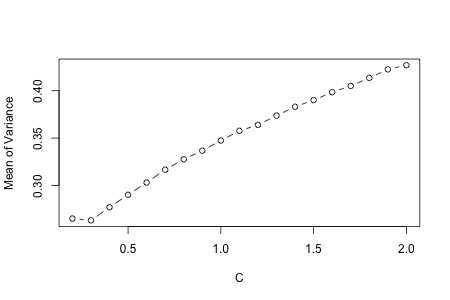
\includegraphics[width=3in]{abb/c_rbf.jpg}}
\caption{The results for chaning Balances linear Datasize 100 Repl 1000 Datasets 20}
\label{fig1}
\end{center}
\end{figure}


\subsection{Influence of the balance of the training dataset}


 Kernels are powerful! Kernels are powerful! Kernels are powerful! Kernels are powerful! Kernels are powerful! Kernels are powerful! Kernels are powerful! Kernels are powerful! Kernels are powerful! Kernels are powerful! Kernels are powerful! Kernels are powerful! Kernels are powerful! Kernels are powerful! Kernels are powerful! Kernels are powerful! Kernels are powerful! Kernels are powerful! Kernels are powerful! Kernels are powerful! Kernels are powerful! Kernels are powerful! Kernels are powerful! Kernels are powerful! Kernels are powerful! Kernels are powerful! Kernels are powerful! Kernels are powerful! Kernels are powerful! Kernels are powerful! Kernels are powerful! Kernels are powerful! Kernels are 

\begin{figure}[!htb]
\begin{center}
\subfloat[]{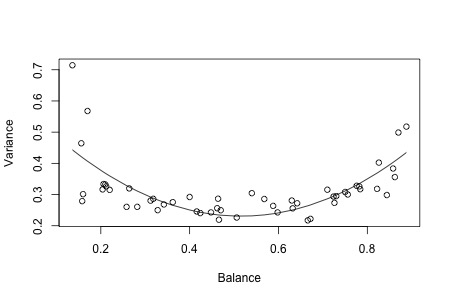
\includegraphics[width=3in]{abb/bal_lin.jpg}}

\subfloat[]{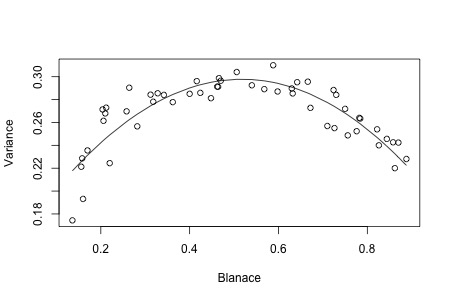
\includegraphics[width=3in]{abb/bal_rbf.jpg}}
\caption{The results for chaning Balances linear Datasize 500 Repl 1000}
\label{fig1}
\end{center}
\end{figure}


\subsection{Influence of the svm attributes}
 Kernels are powerful! Kernels are powerful! Kernels are powerful! Kernels are powerful! Kernels are powerful! Kernels are powerful! Kernels are powerful! Kernels are powerful! Kernels are powerful! Kernels are powerful! Kernels are powerful! Kernels are powerful! Kernels are powerful! Kernels are powerful! Kernels are powerful! Kernels are powerful! Kernels are powerful! Kernels are powerful! Kernels are powerful! Kernels are powerful! Kernels are powerful! Kernels are powerful! Kernels are powerful! Kernels are powerful! Kernels are powerful! Kernels are powerful! Kernels are powerful! Kernels are powerful! Kernels are powerful! Kernels are powerful! Kernels are powerful! Kernels are powerful! Kernels are powerful! 

\begin{figure}[!htb]
\begin{center}
\subfloat[]{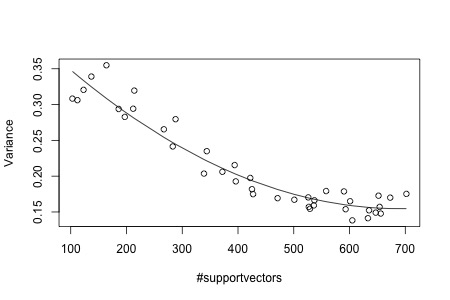
\includegraphics[width=3in]{abb/n_lin.jpg}}

\subfloat[]{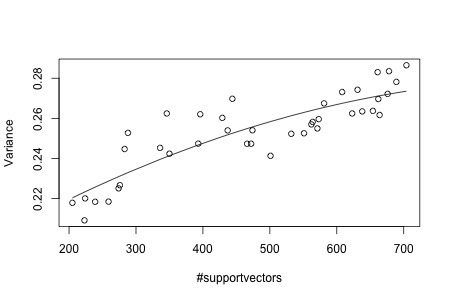
\includegraphics[width=3in]{abb/n_rbf.jpg}}
\caption{The results for chanching number of support vectors Datasize 1000 Repl 500}
\label{fig1}
\end{center}
\end{figure}

 Kernels are powerful! Kernels are powerful! Kernels are powerful! Kernels are powerful! Kernels are powerful! Kernels are powerful! Kernels are powerful! Kernels are powerful! Kernels are powerful! Kernels are powerful! Kernels are powerful! Kernels are powerful! Kernels are powerful! Kernels are powerful! Kernels are powerful! Kernels are powerful! Kernels are powerful! Kernels are powerful! Kernels are powerful! Kern Kernels are powerful! Kernels are powerful! Kernels are powerful! Kernels are powerful! Kernels are powerful! Kernels are powerful! Kernels are powerful! Kernels are powerful! Kernels are powerful! Kernels are powerful! Kernels are powerful! Kernels are powerful! Kernels are powerful! Kernels are powerful! Kernels are powerful! Kernels are powerful! Kernels are powerful! Kernels are powerful! Kernels are powerful! Kernels are powerful! Kernels are powerful! Kernels are powerful! Kernels are powerful! Kernels are powerful! Kernels are powerful! Kernels are powerful! Kernels are powerful! Kernels are powerful! Kernels are powerful! Kernels are powerful! Kernels are powerful! Kernels are powerful! Kernels are 
els are powerful! Kernels are powerful! Kernels are powerful! Kernels are powerful! Kernels are powerful! Kernels are powerful! Kernels are powerful! Kernels are powerful! Kernels are powerful! Kernels are powerful! Kernels are powerful! Kernels are powerful! Kernels are powerful! Kernels are 


\section{Conclusion}
Nice to work with. It also works whit real datasets

Influence of different aspects on variance


C-Parameter: Positive but decreasing influence on variance. Balance of Data: Positive Quadratic influence for Linear and negative quadratic influence for Gaussian SVM. Both with extremum around 0.5 (perfect balance).
Number of support vectors: Positive influence for Gaussian and negative influence for linear SVMs

\section{Outlook}


Analyze the influence of the dimension on variances. Analyze Data simulated from more "exotic" distributions. Analyze influence of other tuning parameters e.g. "Gamma" of RBF-Kernel, degree of Polynomial Kernel etc.




\footnotesize
\bibliographystyle{apalike}
\bibliography{sample}



\end{document}
